(a)\\
\begin{figure}[h]
    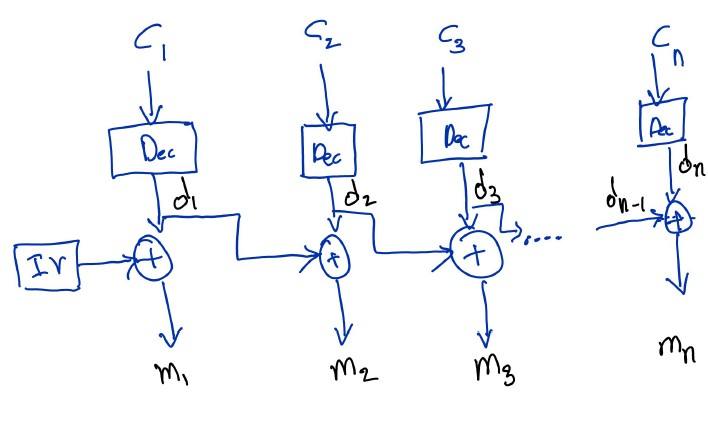
\includegraphics[width=\textwidth,height=\textheight,keepaspectratio]{6-1 Fig1.jpg}
    \caption{Decryption for CBC* mode}
    \centering
\end{figure}\\
(b) As shown in the above figure, let us assume 

\begin{center}
    $d_i$ = Dec ($c_i$) or\\
    $c_i$ = Enc ($d_i$)
\end{center}

As given for CBC*, 

\begin{center}
    $d_1 = m_1 \xor IV $\\
    $d_2 = m_2 \xor d_1 $\\
    i.e., $d_2 = m_2 \xor m_1 \xor IV $\\
    Similarly, $d_3 = m_3 \xor m_2 \xor m_1 \xor IV $\\
\end{center}

The inverse for decryption would be, 

\begin{center}
    $m_1 = d_1 \xor IV $\\
    $m_2 = d_2 \xor d_1 $ ...
\end{center}



To show that this CBC* doesn't have indistinguishable encryptions, 
let us consider message in the format $m = m_1|| m_2||m_3|| ... ||m_n$.\\

Given the Enc is deterministic, the intution of the attack on this CBC* mode was that 
we can recognize repeated blocks in the message.\\

Let us consider IND-EAV adversary, $A$ choose two messages i.e., $m1$ and $m2$ in the below format

\begin{center}
    $m1 = m1_1|| m1_2||m1_3|| ... ||m1_n$\\
    $m1 = m2_1|| m2_2||m2_3|| ... ||m2_n$
\end{center}

And $m1$ is choosen in such a way that $m1_1 ==  m1_2 == m1_3 == ... == m1_n$ and
$m2$ is choosen in such a way that $m2_1 \neq  m2_2 \neq m2_3 \neq ... \neq m2_n$\\

Then 
\begin{center}
    $d1_1 = m1_1 \xor IV $\\
    $d1_2 = m1_2 \xor d1_1 $\\
    i.e., $d1_2 = m1_1 \xor m1_1 \xor IV  = IV$\\
    Similarly, $d1_3 = m1_1 \xor m_1 \xor m1_1 \xor IV = m1_1 \xor IV $\\
\end{center}

As Enc is deterministic, $A$ can distingush $m1$ and $m2$ by checking Enc($m1$) and Enc($m2$) as
\begin{center}
    $c_1 == c_3 == ... == c_i$\\
    $c_2 == c_4 == ...  == c_{i+1}$\\
    where $i$ is an odd number $ \leq n$
\end{center}

If the above check is statisfied then the cipher $c$ corresponds to $m1$. Else it corresponds to $m2$.
With this construction $A$ ouputs 1 if this check is statisfied else 0. This means A always wins CBC* as A runs in polynomial time.
